\documentclass[a4paper, 12pt]{report}

% Packages
\usepackage{xargs}
\usepackage[pdftex,dvipsnames,table]{xcolor}
\usepackage{tocloft}
\usepackage[utf8]{inputenc}
\usepackage[T1]{fontenc}
\usepackage[british,francais]{babel}
\usepackage{lmodern}
\usepackage{graphicx}
\usepackage{float}
\usepackage[pdfpagelabels,%
            urlbordercolor={.909803921569 .796078431373 .552941176471},%
            linkbordercolor={.839215686275 .4862745098 .482352941176},%
            citebordercolor={.839215686275 .607843137255 .447058823529},%
            pdftex,%
            pdfauthor={Alban Chazot},%
            pdftitle={Détection et classification d'objets dans un flux vidéo sphérique},%
            pdfsubject={Rapport de stage de 5A STI},%
            pdfkeywords={réseaux neuronaux, apprentissage profond, traitement de l'image, reconnaissance d'objets, temps réel},%
            pdfproducer={pdfTeX 3.14159265-2.6-1.40.15 (TeX Live 2015/dev/Debian)},%
            pdfcreator={Atom 1.14.3},%
            ]{hyperref}
\usepackage{cleveref}
\usepackage[nonumberlist]{glossaries}
\usepackage{svg}
\usepackage{parskip}
\usepackage{url}
\usepackage{amsmath}
\usepackage{fancyhdr}
\usepackage{vmargin}
\usepackage{sectsty}
\usepackage{listings}
\usepackage{pdfpages}
\usepackage{titling}
\usepackage{lipsum}
\usepackage{microtype}
\usepackage{tabularx}
\usepackage{enumitem}
\usepackage{eurosym}
\usepackage[super]{natbib}
\usepackage[colorinlistoftodos,prependcaption,textsize=tiny]{todonotes}
\usepackage{booktabs} %for rules
\usepackage{multirow}

% Macros
\definecolor{siisky}{HTML}{7AAEDD}
\definecolor{siiblue}{HTML}{0061AA}
\definecolor{siiorange}{HTML}{D64911}
\definecolor{siiorange2}{HTML}{FA6900}
\definecolor{siigrey}{HTML}{333D41}
\definecolor{siigrey2}{HTML}{667074}
\definecolor{siigreen}{HTML}{334100}
\definecolor{siigreen2}{HTML}{667400}
\definecolor{siipurple}{HTML}{8D338A}
\definecolor{siipurple2}{HTML}{C066BD}
\newcommandx{\content}[2][1=]{\todo[linecolor=red,backgroundcolor=red!25,bordercolor=red,#1]{#2}}
\newcommandx{\change}[2][1=]{\todo[linecolor=blue,backgroundcolor=blue!25,bordercolor=blue,#1]{#2}}
\newcommandx{\info}[2][1=]{\todo[linecolor=OliveGreen,backgroundcolor=OliveGreen!25,bordercolor=OliveGreen,#1]{#2}}
\newcommandx{\improvement}[2][1=]{\todo[linecolor=Plum,backgroundcolor=Plum!25,bordercolor=Plum,#1]{#2}}
\newcounter{descriptcount}
\renewcommand{\arraystretch}{1.5}
\newcolumntype{b}{X}
\newcolumntype{s}{>{\hsize=.5\hsize}X}
\newcolumntype{r}{>{\hsize=.2\hsize}X}
\newcommand{\keywords}[1]{\par\textbf{Mot clefs:}\par\quad #1}
\newcommand{\blankpage}{\leavevmode\thispagestyle{empty}\setcounter{page}{0}\newpage}
\newcommand{\nocounter}{\thispagestyle{empty}\setcounter{page}{0}\pagebreak}
\newcommand{\todoref}{\textcolor{red}{\textbf{[REF]}}}

% Document info
\title{Détection et classification d'objets dans un flux vidéo sphérique}
\author{Alban Chazot}
\date{\today}

% Header + footer
\makeatletter
\let\thetitle\@title
\let\theauthor\@author
\let\thedate\@date
\makeatother

% Pages setup
\pagestyle{fancy}
\fancyhf{}
\rhead{\theauthor}
\lhead{\thetitle}
\cfoot{\thepage}
\setmarginsrb{3 cm}{2.5 cm}{3 cm}{2.5 cm}{1 cm}{1.5 cm}{1 cm}{1.5 cm}
\setlength{\parindent}{15pt}
\setcitestyle{super,open={},close={}}
\setlist{nolistsep}
\setlength{\aboverulesep}{0pt}
\setlength{\belowrulesep}{0pt}
\setlength{\extrarowheight}{.0ex}
%\linespread{1.05}

% Glossary
% Magic here
\makeglossaries

\newglossaryentry{lidar}
{
	name={LIDAR},
	description={De l'anglais \emph{LIght Detection And Ranging}, c'est une technique de télémétrie (détermination de la distance d'un objet) qui se base sur la mesure du temps écoulé entre l'émission et la réception d'un faisceau de lumière. Dans notre cas, la source de lumière est un laser émettant de l'infrarouge. Par extension, on nomme LIDAR le dispositif matériel permettant de telles mesures}
}

\newglossaryentry{poc}
{
	name={POC},
	description={\emph{Proof Of Concept}, TODO}
}



% Contents
\begin{document}
{
	% Front page
	\hypersetup{pageanchor=false}
	\nocounter
	
\includepdf[pages={-},offset=30mm -25mm]{premade/frontpage.pdf}
	\nocounter
	\blankpage
	\nocounter
	
	% Abstract
	\begin{otherlanguage}{british}
	\begin{abstract}
		This paper presents the outcome of my internship at SII in the context of my last year of formation in Information Technology Security provided by the institute INSA Centre Val de Loire. This internship falls in line with previous works promoting robotics within the Research \& Development department of the SII Bourges agency.
		\par
		
		\keywords{réseaux neuronaux, apprentissage profond, traitement de l'image, reconnaissance d'objets, temps réel}
	\end{abstract}
\end{otherlanguage}

	\nocounter

	% Thanks
	\section*{Remerciements}
\phantomsection
{
	En prélude à ce rapport, j'aimerais exprimer mes remerciements chaleureux à M. Adel Hafiane, Professeur et Responsable du Laboratoire de Vision par Ordinateurs à l'INSA Centre Val de Loire et Docteur à l'Université du Missouri. J'aimerais particulièrement saluer son implication dans ce projet, tant pour son aide quand à la réalisation du projet que pour sa présence régulière malgrés de nombreux impératifs.
	\par
	Je souhaite remercier M. David Daumand, mon tuteur de stage, Ingénieur Logiciel chez SII, pour avoir su piloter ce projet et y avoir porté une importance telle qu'il puisse être mis en lumière devant des acteurs importants internes et externes à la société. J'aimerais souligner sa volonté de suivre notre équipe de près en dépit du peu de temps dont il disposait.
	\par
	Merci à M. Fabrice Bosch, Directeur de l'agence SII Bourges, pour nous avoir fait confiance quand au choix du matériel à acquérir et pour ses encouragements au long du développement du projet.
	\par
	Finalement, merci à toute l'équipe de l'agence SII Bourges pour leur accueil chaleureux, l'ambiance conviviale des locaux et tous les bons moments passés ensemble.
}

	\nocounter

	% TOC
	\setlength{\cftbeforetoctitleskip}{-7.9em}
	{\footnotesize \tableofcontents}
	\nocounter

	% Introduction
	\hypersetup{pageanchor=true}
	\setcounter{page}{1}
	\section*{Introduction}
\phantomsection
\addcontentsline{toc}{section}{Introduction}
	
	% Contexte
	Ce document relate le travail qui a été effectué au sein du pôle recherche et développement de l'agence de SII Bourges, dans le cadre d'un stage de fin d'études à l'issue de la formation en Sécurité et Technologies Informatique de l'INSA Centre Val de Loire, option Architecture et Sécurité Logicielle.
	
	% Place du projet dans l'entreprise
	La mission s'inscrit dans la continuité du projet robotique du pôle R\&D en coopération avec l'INSA Centre Val de Loire, dont un précédant stage en avait fait l'objet. Cependant, il convient de préciser que le produit présenté ne se base pas sur le précédent travail, si ce n'est dans l'esprit de sa réalisation et de ses objectifs à long terme. En effet, il a pour vocation de faire croître le savoir-faire du pôle face aux problématiques appliquées du traitement du signal et de mettre en avant ces compétences devant des acteurs clés.
	
	% Description du projet
	Le projet est une preuve de concept, dont la finalité répond à la dénomination \emph{Système Robotique Tactique Multi-Missions pour la Surveillance et l'Aide à la Prise de Décision en Milieux à Risques} \gls{robo}. Le système opérationnel final permet de recueillir des informations stratégiques sur l'environnement où il sera déployé, sans mettre en danger des acteurs humains. Ce \gls{poc} a fait l'objet de deux stages dont les sujets sont étroitements liés. Le premier, qui vise à effectuer une cartographie des lieux grâce à un \gls{lidar}, ne sera pas détaillé dans ce rapport. La mission décrite ici consiste principalement à concevoir et implémenter un système de détection et classification d'objets d'intérêt dans un flux vidéo sphérique, ainsi qu'une brique logicielle servant d'interface à la visualisation de ce flux vidéo agrémenté des résultats de la détection.
	
	% Présentation du plan
	\content[inline]{Annonce du plan}

		
	% Chapters
	\chapter{Présentation du contexte}
{
	\section{La Société pour l'Informatique Industrielle}
	{
		\subsection{Acteur de la transformation numérique}
		{
			\par
			{
				SII, ou Société pour l'Informatique Industrielle, est une entreprise de services du numérique implantée dans dix-huit pays au travers de soixante-six agences. Elle propose de multiples services en B2B, dont principalement l'étude et le conseil en technologies sur la maîtrise d'ouvrage de projets et la conception et l'intégration de systèmes.
			}
			
			\begin{figure}[h]
			{
				\centering
				
\includegraphics[page=1,width=.3\textwidth]{figures/logo-sii.pdf}
				\caption{Logo de l'entreprise SII}
				\label{fig:logo-sii}
			}
			\end{figure}
			
			\par
			{
				La fiche signalétique suivante donne une vue d'ensemble de l'entreprise, ainsi qu'elle permet de donner un contexte de réalisation du stage:
			
				\begin{description}
					\item[Nom de l'entreprise:] Société pour l'informatique industrielle (SII)
					\item[Date de création:] 1979\cite{sii_rf}
					\item[Statut juridique:] Société anonyme à directoire et conseil de surveillance
					\item[Siège social:] Paris
					\item[Effectif:] 5949\cite{sii_rs_2017}
					\item[Chiffre d'affaire:] 438,85M\euro\cite{sii_rs_2017}
					\item[Capital:] 103M\euro\cite{sii_rf}
					\item[Direction:] Patrice Demay (directeur général France), Eric Matteucci (président du directoire) et Jean-Paul Chevée (directeur général international)
					\item[Secteurs d'activité:] Aérospatiale, Banque, Défense, Énergie, Finance, Industrie, Média, Télécoms, Transports
					\item[Site internet:] \url{http://www.groupe-sii.com}
				\end{description}
			}
			
			% \begin{figure}
			% 	\centering
			% 	\begin{minipage}{.5\textwidth}
			% 		\centering
			% 		
\includegraphics[page=1,width=0.7\linewidth]{figures/test.pdf}
			% 		\captionof{figure}{Test left}
			% 		\label{fig:Test2}
			% 	\end{minipage}%
			% 	\begin{minipage}{.5\textwidth}
			% 		\centering
			% 		
\includegraphics[page=1,width=0.7\linewidth]{figures/test.pdf}
			% 		\captionof{figure}{Test right}
			% 		\label{fig:Test3}
			% 	\end{minipage}
			% \end{figure}
		}
		\subsection{Historique}
			
			\par
			{
				\change{Trouver une meilleure phrase}
				Quelques dates clefs de l'évolution de l'entreprise:
			}
			
			\begin{description}
			{
				\item[1979:] Création de l'entreprise à Paris par Bernard Huvé, alors ingénieur consultant.
				\item[1984:] À l'occasion d'un contrat avec le laboratoire d'IBM, une deuxième agence est ouverte à nice.
				\item[1987-1989:] Déploiement de SII en Île-de-France avec la création des deux agences de Cergy Pontoise et Vélizy.
				\item[1992:] À la suite d'évolutions importantes du secteur de l'informatique, l'entreprise se recentre sur l'assistance technique et obtient la certification ISO 9001.
				\item[1997:] Ouverture des agences de Rennes et Aix-en-Provence.
				\item[1999:] Introduction en bourse de l'entreprise.
				\item[2000-2007:] Accroissement du maillage national: ouverture d'agences à Bordeaux, Brest, Caen, La Ciotat, Lannion, Le Mans, Lyon, Niort, Montpellier, Tours et Vitrolles. Ouverture de filiales internationales en République Tchèque et en Pologne.
				\item[2010:] Acquisition de AIDA Development, société allemande, qui permet à l'entreprise de pénétrer le premier marché européen.
				\item[2015:] Implantation aux Pays-Bas et en Colombie.
				\item[2016:] Implantation aux Canada et en Angleterre.
			}
			\end{description}
	}
	\section{Développement et exposition du savoir-faire}
	
		\subsection{SII Research et le pôle robotique}
			
			\par
			{
				SII
			}
			\par
			{
				\info{Ceci est un copié/collé pur pour servir de base}
				Nous avons également créé SII Research dans un objectif de structurer et de fédérer la totalité de nos innovations technologiques. Au-delà des clients, ce projet est enthousiasmant pour l’ensemble de nos équipes puisqu’il est au cœur de ce qui constitue l’ADN du métier de l’ingénieur. Et plus encore, il renforce ce qui est notre slogan depuis le début : SII, le partenaire technologique.
			}
			\par
			
		\subsection{Technologies de pointe}
		
			\lipsum[10-12]
			
}

	\chapter{Un système de détection omnidirectionnel en temps réel}

	\section{Analyse du besoin}

		\subsection{Le concept du système}
			
			% Idée globale du système
			Le projet vise à créer un démonstrateur d'un concept plus large, à savoir un système permettant de piloter un ensemble de robots et d'exploiter les informations issues de leurs périphériques de capture afin d'effectuer des missions de reconnaissance sans déployer de troupes au sol, et risquer de mettre leurs vies en dangers sur des terrains potentiellement à risques. Ce démonstrateur illustre donc la faisabilité de ce concept, mais d'une manière plus limitée. Le but est de développer un système opérationnel pour un seul robot équipé d'un \gls{lidar} et d'une caméra sphérique, permettant de contrôler ses déplacements, d'analyser les données acquises par ces deux périphériques, et d'afficher les résultats de ces traitements dans une interface utilisateur.
			\par
			% Mon sujet de stage
			Devant l'ampleur du travail à accomplir, le projet a été scindé en deux sujets de stage, chacun correspondant au traitement des données acquise par un des deux périphériques. Le sujet dont il est question dans ce document est relatif à l'exploitation de la caméra sphérique. On dégage trois objectifs principaux à la mission décrite dans le sujet du stage:
			\begin{itemize}[noitemsep]
				\item Réalisation d'un état de l'art permettant de choisir le matériel et l'algorithme à utiliser.
				\item Développement d'une brique logicielle permettant d'effectuer de la reconnaissance d'objets en temps réel.
				\item Développement d'une brique logicielle permettant d'afficher les résultats de la détection incrustés à la vidéo.
			\end{itemize}
			\par
			Préalablement à la conception architecturale du projet, un document de \improvement{ajouter ref annexe + corriger STBL}\emph{Spécification Technique du Besoin Logiciel (STBL)} a été réalisé afin de détailler ces trois objectifs et de référencer les exigences de qualité. A cette occasion, des éléments d'analyse fonctionnelle ont été menés afin de mieux cerner le besoin. Le diagramme de cas d'utilisation suivant (\autoref{fig:usecase}) définit les exigences fonctionnelles et le cadre du projet d'un point de vue de l'utilisateur.
			
			\begin{figure}[h]
			{
				\centering
				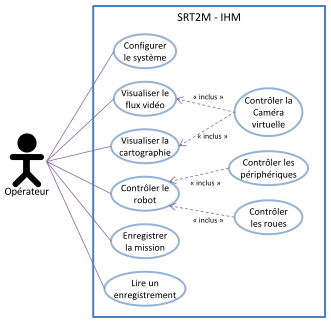
\includegraphics[page=1,width=0.7\textwidth]{figures/usecase.pdf}
				\caption{Diagramme de cas d'utilisation de l'interface homme-machine}
				\label{fig:usecase}
			}
			\end{figure}

			\improvement[inline]{Ajouter justification des technos employées}


		\subsection{Exigences}

			Le document de Spécification Technique du Besoin Logiciel développe le fonctionnement de la brique logicielle en trois fonctions principales détaillées dans la liste suivante, accompagnées de leurs descriptions:
			\begin{description}[noitemsep, before={\setcounter{descriptcount}{0}},font=\bfseries\stepcounter{descriptcount}\thedescriptcount.~]
				\item[Acquisition Vidéo:] Acquérir un flux vidéo provenant d’une caméra \oldstylenums{360}\degre.
				\item[Détection:] Détecter et classifier les objets d’intérêt présents dans le flux vidéo.
				\item[Retour visuel:] Offrir un retour visuel à l’opérateur présentant le flux vidéo et les objets détectés.
			\end{description}
			Ce document précise ces fonctions en y faisant correspondre des facteurs de qualité, appelés \emph{exigences fonctionnelles} qui permettent de piloter la réalisation du produit présentant ces fonctionnalités. Elles sont recensées dans les tableaux suivants avec leur référence, leur intitulé et une courte description:
			
			\begin{center}
	\begin{tabularx}{\textwidth}[t]{rsb}

		\arrayrulecolor{green}\hline
		\multicolumn{3}{c}{\textbf{\textcolor{myGreen}{FNC001-ACQUISITION\_VIDEO}}}\\
		\hline

		\textbf{Référence} & \textbf{Intitulé} & \textbf{Description} \\
		\arrayrulecolor{black}\hline
		
		FNC001\_01 & Décoder le flux vidéo & Le flux doit être décomposé en images séparées au format RGB8 \\
		\arrayrulecolor{gray}\hline
		FNC001\_02 & Transmettre séquentiellement les images obtenues du décodage & Les images décodées doivent être mises à disposition des fonctions dépendantes (détection et retour visuel) dans l’ordre d’obtention et sans latence supérieure à la vitesse d’acquisition. \\
		\arrayrulecolor{gray}\hline
		FNC001\_03 & Transmettre un horodatage relatif à une image décodée & Chaque image mise à disposition doit être accompagnée d’un horodatage permettant de la situer dans le temps de manière cohérente. \\
		\arrayrulecolor{gray}\hline
		FNC001\_04 & Relayer l’état du matériel et de la connexion & Les informations suivantes doivent être mises à disposition de la fonction retour visuel: Caméra connectée, flux vidéo disponible, erreur de décodage \\
		\arrayrulecolor{gray}\hline
		FNC001\_05 & Traiter les éventuelles erreurs de décodage & Les erreurs temporaires ne doivent pas affecter le fonctionnement du logiciel. En cas d’erreur, la relayer au retour visuel. \\
		\arrayrulecolor{gray}\hline

		\arrayrulecolor{green}\hline
		\multicolumn{3}{c}{\textbf{\textcolor{myGreen}{FNC002-DETECTION}}}\\
		\hline

	\end{tabularx}

	\begin{tabularx}{\textwidth}[t]{rsb}

		\textbf{Référence} & \textbf{Intitulé} & \textbf{Description} \\
		\arrayrulecolor{black}\hline
		
		FNC001\_01 & Décoder le flux vidéo & Le flux doit être décomposé en images séparées au format RGB8 \\
		\arrayrulecolor{gray}\hline
		FNC001\_02 & Transmettre séquentiellement les images obtenues du décodage & Les images décodées doivent être mises à disposition des fonctions dépendantes (détection et retour visuel) dans l’ordre d’obtention et sans latence supérieure à la vitesse d’acquisition. \\
		\arrayrulecolor{gray}\hline
		FNC001\_03 & Transmettre un horodatage relatif à une image décodée & Chaque image mise à disposition doit être accompagnée d’un horodatage permettant de la situer dans le temps de manière cohérente. \\
		\arrayrulecolor{gray}\hline
		FNC001\_04 & Relayer l’état du matériel et de la connexion & Les informations suivantes doivent être mises à disposition de la fonction retour visuel: Caméra connectée, flux vidéo disponible, erreur de décodage \\
		\arrayrulecolor{gray}\hline
		FNC001\_05 & Traiter les éventuelles erreurs de décodage & Les erreurs temporaires ne doivent pas affecter le fonctionnement du logiciel. En cas d’erreur, la relayer au retour visuel. \\
		\arrayrulecolor{gray}\hline
		
	\end{tabularx}

	\begin{tabularx}{\textwidth}[t]{rsb}

		\arrayrulecolor{green}\hline
		\multicolumn{3}{c}{\textbf{\textcolor{myGreen}{FNC003-RETOUR\_VISUEL}}}\\
		\hline

		\textbf{Référence} & \textbf{Intitulé} & \textbf{Description} \\
		\arrayrulecolor{black}\hline
		
		FNC001\_01 & Décoder le flux vidéo & Le flux doit être décomposé en images séparées au format RGB8 \\
		\arrayrulecolor{gray}\hline
		FNC001\_02 & Transmettre séquentiellement les images obtenues du décodage & Les images décodées doivent être mises à disposition des fonctions dépendantes (détection et retour visuel) dans l’ordre d’obtention et sans latence supérieure à la vitesse d’acquisition. \\
		\arrayrulecolor{gray}\hline
		FNC001\_03 & Transmettre un horodatage relatif à une image décodée & Chaque image mise à disposition doit être accompagnée d’un horodatage permettant de la situer dans le temps de manière cohérente. \\
		\arrayrulecolor{gray}\hline
		FNC001\_04 & Relayer l’état du matériel et de la connexion & Les informations suivantes doivent être mises à disposition de la fonction retour visuel: Caméra connectée, flux vidéo disponible, erreur de décodage \\
		\arrayrulecolor{gray}\hline
		FNC001\_05 & Traiter les éventuelles erreurs de décodage & Les erreurs temporaires ne doivent pas affecter le fonctionnement du logiciel. En cas d’erreur, la relayer au retour visuel. \\
		\arrayrulecolor{gray}\hline

	\end{tabularx}
\end{center}

			\bigskip

			La spécification technique décrit aussi d'autres contraintes de réalisation et de qualité, plus décorrélées de l'expression du besoin, qui auront un impact sur les décisions de conception et d'architecture du produit final. Pilotant l'ensemble de la réalisation, elles ne disposent pas de fonctions précises qui leur répondent, et de ce fait n'ont pas de référence. Ces contraintes sont énumérées dans les tableaux suivants:
			
			\begin{center}
	\scriptsize
	\begin{tabularx}{\textwidth}[t]{rsb}
		\arrayrulecolor{siiorange2}\cmidrule(l){1-3}
		\multicolumn{3}{c}{\textbf{\textcolor{siiorange}{Contraintes d'environnement}}}\\
		\arrayrulecolor{siiorange2}\cmidrule(l){1-3}

		\textbf{Type} & \textbf{Élément} & \textbf{Composants} \\
		\arrayrulecolor{black}\cmidrule(l){1-3}
		
		\multirow{4}{*}{Matériel} & \multirow{2}{*}{Plateforme mobile} & Raspberri Pi 3b \\ \arrayrulecolor{gray}\cmidrule(l){3-3}
		                          &                                    & périphérique d’acquisition de flux vidéo \\ \arrayrulecolor{gray}\cmidrule(l){2-3}
		                          & \multirow{2}{*}{Poste de contrôle} & Périphériques d'interface \\ \arrayrulecolor{gray}\cmidrule(l){3-3}
		                          &                                    & Processeur graphique \\ \arrayrulecolor{gray}\cmidrule(l){1-3}
		\multirow{7}{*}{Logiciel} & \multirow{3}{*}{Plateforme mobile} & Noyau linux (ARM) \\ \arrayrulecolor{gray}\cmidrule(l){3-3}
		                          &                                    & Outils GNU \\ \arrayrulecolor{gray}\cmidrule(l){3-3}
		                          &                                    & Framework ROS \\ \arrayrulecolor{gray}\cmidrule(l){2-3}
		                          & \multirow{4}{*}{Poste de contrôle} & Noyau Linux (x86-64) \\ \arrayrulecolor{gray}\cmidrule(l){3-3}
		                          &                                    & Outils GNU \\ \arrayrulecolor{gray}\cmidrule(l){3-3}
		                          &                                    & Framework ROS \\ \arrayrulecolor{gray}\cmidrule(l){3-3}
		                          &                                    & CUDA \\ \arrayrulecolor{gray}\cmidrule(l){1-3}
	\end{tabularx}
	
	\begin{tabularx}{\textwidth}[t]{rsb}
		\arrayrulecolor{siigreen2}\cmidrule(l){1-3}
		\multicolumn{3}{c}{\textbf{\textcolor{siigreen}{Contraintes d'interface}}}\\
		\arrayrulecolor{siigreen2}\cmidrule(l){1-3}

		\textbf{Type} & \textbf{Élément} & \textbf{Détails} \\
		\arrayrulecolor{black}\cmidrule(l){1-3}
		
		\multirow{4}{*}{Matériel} & \multirow{4}{*}{Périphérique d'acquisition vidéo} & Connection \gls{usb} 3.0\\ \arrayrulecolor{gray}\cmidrule(l){3-3}
								  &                                                   & Format vidéo \gls{mjpeg} \\ \arrayrulecolor{gray}\cmidrule(l){3-3}
								  &                                                   & Protocole \gls{uvc} \\ \arrayrulecolor{gray}\cmidrule(l){3-3}
								  &                                                   & Format d'image "Dual Fisheye" \\ \arrayrulecolor{gray}\cmidrule(l){1-3}
		\multirow{6}{*}{Logiciel} & \multirow{6}{*}{Système Robotique}                & Interface avec \gls{ros} \\ \arrayrulecolor{gray}\cmidrule(l){3-3}
								  &                                                   & Execution simultanée (les traitements ne doivent pas bloquer le reste du système) \\ \arrayrulecolor{gray}\cmidrule(l){3-3}
								  &                                                   & Latence minime dans le transfert d'images (<200ms) \\ \arrayrulecolor{gray}\cmidrule(l){3-3}
								  &                                                   & Transfert des détections synchronisé avec les images \\ \arrayrulecolor{gray}\cmidrule(l){3-3}
								  &                                                   & Transfert des données selon un protocole à définir \\ \arrayrulecolor{gray}\cmidrule(l){1-3}
	\end{tabularx}

	\begin{tabularx}{\textwidth}[t]{sb}
		\arrayrulecolor{siipurple2}\cmidrule(l){1-2}
		\multicolumn{2}{c}{\textbf{\textcolor{siipurple}{Contraintes de programmation}}}\\
		\arrayrulecolor{siipurple2}\cmidrule(l){1-2}

		\textbf{Élément} & \textbf{Valeur} \\
		\arrayrulecolor{black}\cmidrule(l){1-2}
		
		\multirow{1}{*}{Langages}   & C++ \\ \arrayrulecolor{gray}\cmidrule(l){1-2}
		\multirow{3}{*}{Frameworks} & \gls{cuda} \\ \arrayrulecolor{gray}\cmidrule(l){2-2}
								    & Qt5 \\ \arrayrulecolor{gray}\cmidrule(l){2-2}
									& \gls{ros} \\ \arrayrulecolor{gray}\cmidrule(l){1-2}
	\end{tabularx}
	
\end{center}

			
			\improvement[inline]{Ajouter du contenu ?}

	\section{Etat de l'art}

		\subsection{Détection d'objets et apprentissage automatique}
			
			La détection d'objets d'intérêt est une discipline de la vision par ordinateur qui consiste à détecter la présence d'un type d'objet (appelé communément \emph{classe}) dans une image. On peut distinguer plusieurs problématiques issues du sujet:
			\begin{description}[noitemsep]
				\item[Localisation:] Trouver les coordonnées exactes d'un objet dans une image.
				\item[Classification:] Associer une image contenant un objet à un élément d'un ensemble de classes prédéfinies.
				\item[Reconnaissance:] Identifier une instance précise d'une classe (distinguer deux éléments distincts de même classe).
			\end{description}
			Pour répondre à ces problématiques, on utilise généralement un \emph{système de reconnaissance de forme}, procédé permettant de décrire une image ou partie d'une image au travers d'une représentation mathématique et de la comparer à des modèles de représentations connus afin de l'assimiler à une classe définie. Un des exemples les plus connus est la \emph{Méthode de Viola et Jones}\cite{viola}, principalement utilisée pour la détection de visages. Ces systèmes comprennent deux éléments principaux:
			\begin{itemize}[noitemsep]
				\item Un extracteur des caractéristiques de l'entrée
				\item Un classifieur qui associe l'entrée à une classe
			\end{itemize}
			\par
			L'extracteur de caractéristiques est un algorithme qui permet de traduire une image, ou partie d'une image, en une représentation mathématique de caractéristiques visuelles qu'elle contient (coins, traits, points, dégradés \dots). L'approche classique consiste à considérer l'entrée comme un élément d'un espace vectoriel de dimension $n_{0}$ et d'y appliquer une fonction mathématique pour obtenir un résultat appartenant à un espace vectoriel de dimension $n_{1}$ avec $n_{1} < n_{0}$, qu'on appelle \emph{vecteur de caractéristiques} ou \emph{descripteur}. L'intérêt de ces traitements réside dans cette réduction de dimensions, qui constitue en quelque sorte un résumé de la donnée, et permet de distinguer plus facilement des classes grâce à l'algorithme de classification. Il existe de nombreux algorithmes extracteurs de caractéristiques, autant qu'il existe de nombreux moyens de décrire les caractéristiques visuelles d'une image. Citons les algorithmes \emph{SIFT}\cite{sift}, \emph{HOG}\cite{hog} et \emph{SURF}\cite{surf} comme exemples, par leur utilisation régulière dans la communauté du traitement du signal. Contrairement au classifieur, ces algorithmes sont fixes, c'est à dire que pour une même entrée, ils produiront toujours la même sortie.
			\par
			Le classifieur, souvent basé sur des \emph{Machines à Vecteur de Support}\cite{svm}, permet de discriminer des groupes au sein des résultats, et donc de déterminer l'appartenance d'un résultat à une classe. Afin de déterminer la classe résultante d'un objet ($y_{i}$), il effectue des sommes pondérées des composantes de ses vecteurs de caractéristiques, et les compare à des valeurs seuils permettant d'activer ou non une sortie. Un algorithme classifieur est généralement entraînable, c'est à dire qu'en lui fournissant un ensemble de couples (vecteurs de caractéristiques; résultat attendu $\hat{y}_{i}$) il déterminera lui même la loi permettant de les séparer. L'enjeu est de réduire l'écart entre $y$ et $\hat{y}$, cette phase d'entraînement revient donc à minimiser une fonction objectif en modulant les pondérations des sommes ($\theta_{i}$) jusqu'à obtenir une loi de discrimination optimale. Un tel comportement correspond à un apprentissage supervisé, où la réponse correcte est connue, permettant à la machine de s'améliorer. Une fois cette phase achevée, le système est théoriquement apte à classifier avec exactitude de nouvelles entrées, jusqu'alors inconnues.

		\subsection{Apprentissage profond et R-CNN}

			L'apprentissage profond est basé sur l'utilisation de réseaux neuronaux artificiels multicouche. Ces réseaux sont schématiquement inspirés des réseaux neuronaux biologiques tels que nous les connaissons en ceci qu'ils se basent sur la transmission de données entre de nombreux modules, appelés \emph{Neurones Formels}, illustré en \autoref{fig:aneuron}. Ces modules prennent en entrée $x_{i}$ des valeurs issues des résultats de neurones précédents ou bien de l'entrée d'origine du système. Ces entrées sont ensuite sommées avec leur \emph{poid synaptique} $\theta_{i}$ respectif, ainsi qu’un coefficient $\theta_{0}$ appelé biais. Ce résultat pondéré est ensuite transmis à une fonction d’activation non linéaire. Celle-ci activera la synapse suivante (ici, la sortie), si son résultat dépasse un seuil donné.
			\begin{figure}[h]
			{
				\centering
				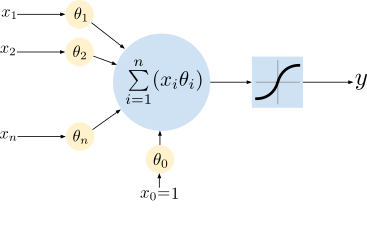
\includegraphics[page=1,width=.6\textwidth]{figures/aneuron.pdf}
				\caption{Schéma d'un neurone formel}
				\label{fig:aneuron}
			}
			\end{figure}
			
			
			\info[inline]{WIP}

		\subsection{Vidéo sphérique}
			% de 1 à 36 objectifs
			La photographie sphérique, aussi connue sous le nom de photographie à 360\degre ou \emph{VR photography} (pour réalité virtuelle), s'apparente à la photographie panoramique, en ceci qu'elle vise à capturer un point de vue sous la forme d'une image avec un champ de vision exceptionnellement large (ratio supérieur à $1:2$)\cite{fnumpano}. En effet, le but est de représenter une scène complète dans une seule image, comme on pourrait l'observer en effectuant un tour complet autour d'un point fixe. Le concept s'est fortement démocratisé au travers de son apparition dans \emph{Google StreetView}, et plus récemment par l'importante médiatisation de la réalité virtuelle, permettant une plus grande immersion lors du visionnage de photographies ou de vidéos sphériques.
			\par
			L'obtention d'une image prête au visionnage n'est théoriquement pas possible avec une seule prise de vue. Les techniques utilisées pour obtenir de telles images reposent toutes sur l'assemblage de plusieurs photographies, ce qui peut faire apparaître des incohérences dans la scène lorsqu'elles sont prises à des temps différents (les sujets qui se déplacent peuvent être présents sur plusieurs photographies, donc plusieurs parties de la scène). Pour obtenir le plus de cohérence dans le flux vidéo et minimiser le traitement dû à l'assemblage, il a donc été décidé d'acquérir un appareil qui permet de capturer instantanément une scène complète avec plusieurs objectifs.
			\improvement[inline]{Ajouter images ou schémas}
			\par
			Cette médiatisation importante de la réalité virtuelle a entraîné la conception de caméras à \oldstylenums{360}\degre par de nombreux fabricants grand-public (LG, Samsung, Kodak), par opposition aux fabricants de matériel vidéo professionnel, comme FLIR (avec sa série des \emph{Ladybug} \cite{ladybug}). La recherche de matériel à acquérir s'est donc concrétisée par la création d'un comparatif des différentes caméras à \oldstylenums{360}\degre présent dans l'annexe \todoref.
			
			Le choix d'acquisition du matériel à été piloté principalement par les facteurs suivants:
			\begin{itemize}[noitemsep]
				\item Couverture spatiale complète ($360^{\circ}\times180^{\circ}$)
				\item Au moins \oldstylenums{15} images/secondes
				\item Transmission de la vidéo par WiFi ou USB
				\item Transmission de la capture vidéo en temps réel
				\item Assemblage d'image en temps réel
				\item Qualité d'image correcte (subjectif)
				\item Point de montage par vis
				\item Prix ne dépassant pas 500\euro
			\end{itemize}
			
			Notre choix s'est d'abord porté sur le produit Insta\oldstylenums{360} 4K\cite{insta360}, qui possède un système d'assemblage en temps réel intégré et une très bonne qualité d'image. Cependant, le produit n'étant pas disponible au moment de l'achat, nous avons dûs nous reporter sur la caméra Theta S de Ricoh\cite{ricohthetas}, possédant une qualité d'image moindre et aucun moyen natif d'assemblage en temps réel sous systèmes linux. Ce dernier point s'est avéré crucial dans l'organisation du travail, car il a nécessité une charge de travail importante, détaillée en \ref{sub:transfo}.

	\section{Problématiques soulevées}

		\subsection{Détection sur une image déformée}

			\content[inline]{A faire}

		\subsection{Visualisation des résultats}

			\content[inline]{A faire}
		
			

	\chapter{Conception et développement}

	\section{Architecture du logiciel}

		\subsection{Vision globale}
			
			D'un point de vue matériel, le projet est séparé en deux parties: la plateforme mobile, robot sur lesquels sont connectés les périphériques de capture, et le poste de contrôle, terminal de consultation des informations par l'opérateur humain. Cette architecture simple se retrouve dans le schéma \todoref.
			\change[inline]{Ajouter schéma archi wifibot[camera,lidar,rpi] <-> poste contrôle[pc,hid,ecran]}
			\par
			La plateforme mobile est un \emph{WiFiBot Lab V3}\cite{wifibot}, fourni par l'INSA Centre-Val-de-Loire, dont la carte de contrôle, munie d'un processeur x86, fonctionne sous \emph{Windows XP Embedded} et dispose d'un serveur connecté par WiFi à un routeur (fourni également) permettant de lui envoyer des commandes de contrôle des moteurs des roues. Dans un souci de conservation de l'existant et par simplicité de développement, nous avons choisi de contrôler les périphériques et de centraliser les transfers de données au travers d'un \emph{Raspberry Pi 3b}, qui possède une puissance de calcul raisonnable face à sa faible consommation et une carte WiFi intégré. Par ailleurs, le fait que micro-ordinateur fonctionne sous \emph{Linux} nous permet de conserver une continuité dans le choix des technologies logicielles à utiliser.
			\par
			Le poste de contrôle, connecté au même routeur que le WifiBot, est constitué d'un micro-ordinateur disposant d'un \gls{gpu} dédié (NVIDIA K620), d'un écran et de périphériques d'entrées standard (clavier, souris), permettant d'intéragir avec l'opérateur. Au vu de la faible puissance de calcul dont dispose la plateforme mobile, le choix a été fait de centraliser les traitements lourds sur ce poste.
			\par
			Le logiciel se scinde en deux parties bien distinctes:
			\begin{description}[noitemsep]
				\item[l'Interface Homme-Machine], qui permet à l'opérateur de contrôler les mouvements de la plateforme mobile, démarrer les périphériques de capture et leurs chaînes de traitement, d'enregistrer une mission et de visionner le déroulement d'une mission enregistrée.
				\item[le réseau de traitement de données], qui permet d'exploiter les données en sortie des périphériques de capture de manière à en tirer des informations pertinentes: la cartographie des lieux visités et les objets d'intérêt qui y sont présents.
			\end{description}
			Cette architecture se retrouve en \todoref, avec des éléments détaillant le fonctionnement de chaque partie.
			\change[inline]{Ajouter schéma archi logiciel général}

		\subsection{Réseau de traitement de données}

			\change[inline]{Ajouter schéma réseau ros}
			\content[inline]{A faire}
			
		\subsection{Interface Homme-Machine}
		\label{sub:ihm}

			\change[inline]{Ajouter schéma archi ihm}
			\content[inline]{A faire}

	\section{Détails d'implémentation}
	
		\subsection{Transmission de la vidéo}
		
			La caméra Ricoh Theta S comporte une carte WiFi, ce qui permet, pour une utilisation \og normale \fg{} (avec l'application Android fournisseur) de s'y connecter avec un téléphone fonctionnant sous Android, afin d'y transférer les données de la caméra. Ces données peuvent prendre la forme de photos ou de vidéos, préalablement enregistrées sur la mémoire interne de la caméra et donc récupérées en différé, ou d'un mode spécial, nommé \emph{live}, qui permet de transmettre un flux vidéo continu correspondant à la capture des objectifs de la caméra en temps réel. Ce mode permet de transmettre un aperçu au téléphone avant de prendre une photo, uniquement supporté par l'application Android du fabricant. Devant la demande croissante du public d'utiliser ce mode de \og livestream \fg{}, les développeurs ont choisi de le rendre disponible sur pc, au travers d'un pilote matériel permettant aux OS \emph{Windows} et \emph{Mac OS} de considérer la caméra, alors branchée à l'ordinateur par \gls{usb}, comme une webcam, permettant ainsi la plupart des programmes d'exploiter ce flux vidéo. Ce pilote se charge de communiquer avec le bon protocole les commandes utilisateurs à la caméra et de transformer le flux vidéo dans un format exploitable. Après analyse du pilote windows, il a été découvert (car non exprimé dans la documentation du produit) qu'il utilise la bibliothèque \emph{libUVC}, et donc que la communication avec la caméra est effectuée au travers du protocole \gls{uvc}. La caméra étant sur la plateforme mobile disposant d'un \emph{Raspberry Pi 3b}, il a été développé un noeud \gls{ros} permettant de lui envoyer des commandes, d'acquérir le flux vidéo direct et de l'envoyer sur le poste de contrôle.
			\par
			Une problématique arrivée rapidement est celle de la transmission sur le WiFi.
			La Raspberry Pi dispose d'une carte WiFi qui ne supporte que la norme 802.11g, et ne peut donc transférer des données qu'au débit réel maximal de 25 Mb/s.
			Après une analyse de paquet en cas réel, la bande passante disponible pour le flux vidéo n'est que de 17,6 Mb/s, soit 2,2 Mo/s.
			Une image \gls{jpeg} en sortie de la caméra pèse en moyenne 400ko, et la caméra opère à 15 images/s, ce qui nécessite un débit de 6M/s.
			La Raspberri Pi dispose d'un \gls{gpu} \emph{VideoCore IV}\cite{videocore}, servant en priorité à encoder et décoder des vidéos (par exemple, pour lire un flux vidéo en haute qualité depuis internet).
			Il est donc possible d'utiliser la bibliothèque \emph{OpenMAX} pour encoder une vidéo, qui devrait donc peser moins qu'une séquence d'images décorrélées.
			Cependant, après de nombreux éssais d'envoi de flux converti (au format h264, le format le plus optimisé pour cette puce graphique), il s'est avéré que l'encodage entraîne un surplus de traitement au niveau du processeur de la Raspberry, qui entraîne l'introduction d'une latence importante entre la capture d'une image et sa visualisation sur le poste opérateur.
			Il a donc été décidé de réduire la vitesse du flux de la caméra à 5 images/s, afin de ne nécessiter que 2Mo/s de bande passante.
			%1 jpeg 1280x768 = 400ko
			% 5 fps = 2000ko/s
			%15 fps = 6000ko/s
			%wifi        54   mb/s | 6.75  mo/s
			%            25   mb/s | 3.125 mo/s
			%benchmarks: 17.6 mb/s | 2.2   mo/s
			\par
			Les images sont donc extraites des paquets \gls{usb} et envoyées au poste de contrôle encapsulées dans un protocole simple et efficace pour la transmission de données unidirectionnelle en temps réel, dont l'unité de donnée (\gls{pdu}) est la suivante:

			\begin{center}
				\scriptsize
				\begin{tabularx}{\textwidth}[h]{|Y|Y||Y|}
					\toprule
					\multicolumn{2}{|c||}{entête (24 octets)} & charge utile (variable) \\
					\midrule
					Identifiant protocole (8 octets) & taille image (16 octets) & données (variable)\\
					\bottomrule
				\end{tabularx}
			\end{center}

			Ces trames sont encapsulées dans des trames \gls{tcp} pour laisser le système s'occupper de la fragmentation et de l'ordonnacement, ce qui simplifie le traitement du côté réception et du côté traitement des données (pas de mise en file d'attente).
			
		\subsection{Transformation vidéo}
		\label{sub:transfo}
		
			En sortie de la caméra, l'image correspond aux photos prises par les deux objectifs, chacun ayant un angle de prise de vue de $190^{\circ}$, horizontalement et verticalement, et chacun étant de type \gls{fisheye} circulaire. Un exemple d'image non traitée est représenté \autoref{fig:rawcapture}. Le fait de disposer de deux photos \gls{fisheye} qui couvrent l'ensemble du point de vue à la position de la caméra s'appelle couramment \emph{Dual Fisheye}. On peut parler de représentation sphérique d'un point de vue, l'angle de champ étant de $360^{\circ}\times180^{\circ}$. Les caractéristiques spatiales visibles observent un niveau de déformation proportionnel à leur éloignement du centre de l'objectif. À défaut de traitement, la détection et la classification des objects contenus dans la scène présentent des imprécisions qui rendent de tels résultats inexploitables.
			\begin{figure}[h]
			{
				\centering
				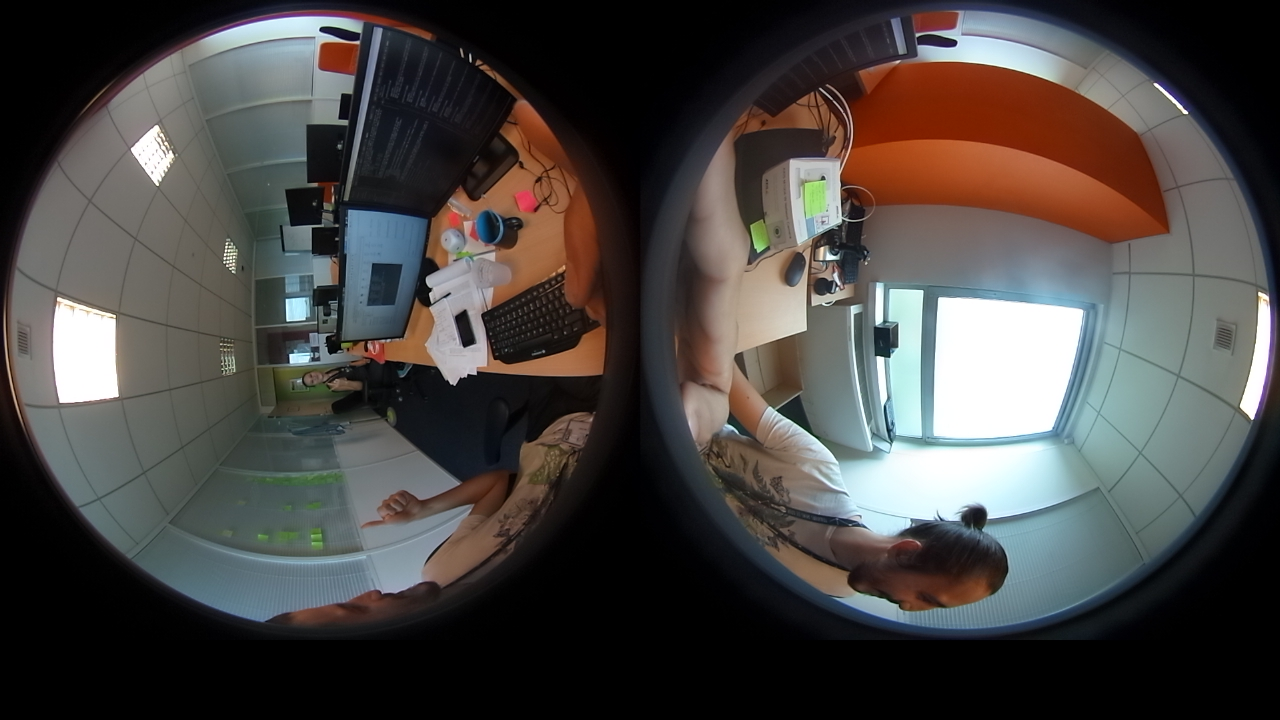
\includegraphics[width=1\textwidth]{figures/capture.jpg}
				\caption{Image non traitée capturée en sortie de la caméra}
				\label{fig:rawcapture}
			}
			\end{figure}
			\par
			Comme évoqué dans la section précédente, le pilote fourni par le fabricant transforme cette image en appliquant une projection spatiale sur chacun de ses pixels de manière à obtenir une couverture complète du point de vue en projection équirectangulaire. Cette méthode permet de voir l'intégralité de la surface d'une sphère sur un plan. Les figures suivantes visent à illustrer cette opération.
			\par
			On considère la scène \autoref{fig:cage}, où notre point de vue correspond à la sphère rouge. Notre scène comporte donc une cage dont les faces ont des couleurs différentes et des numéros permettant de mettre les caractéristiques spatiales en valeur.
			\begin{figure}[h]
			{
				\centering
				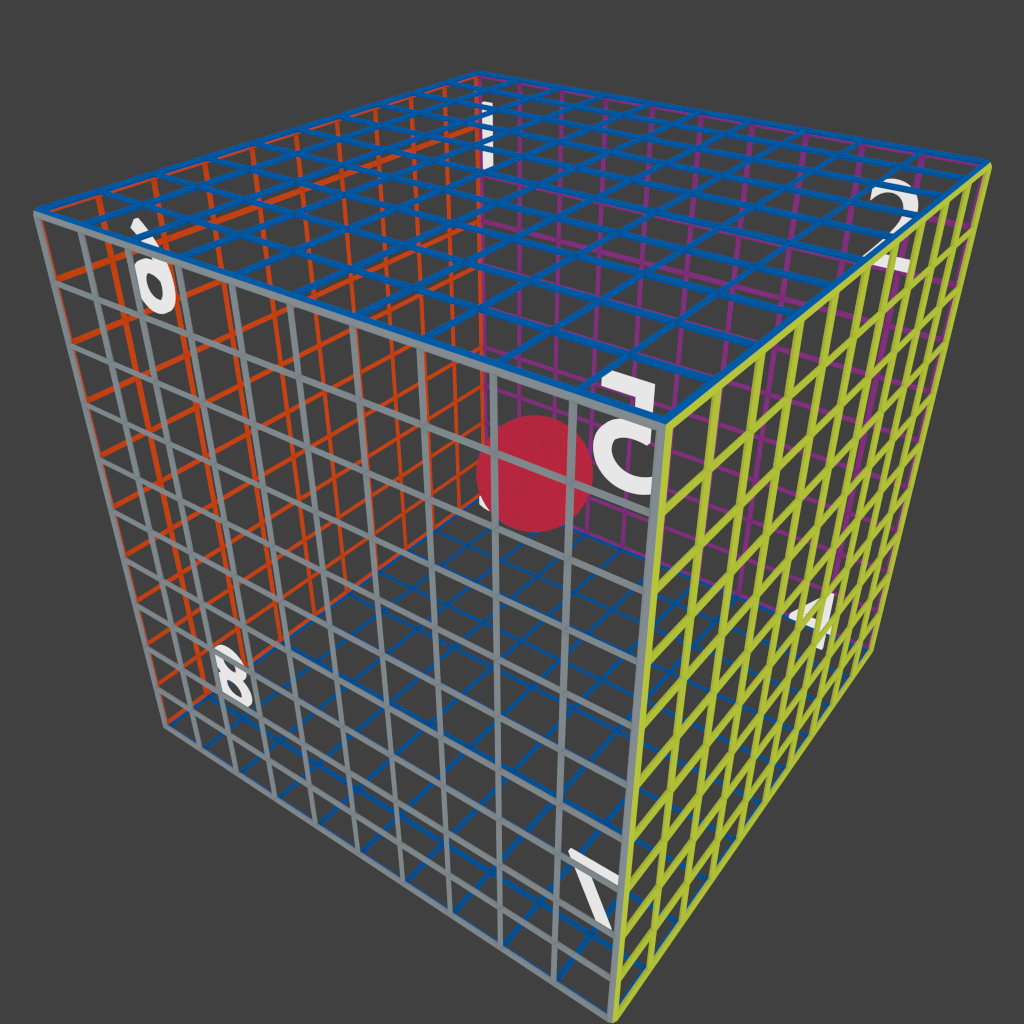
\includegraphics[width=0.6\textwidth]{figures/cage.png}
				\caption{Scène d'exemple vue de l'extérieur}
				\label{fig:cage}
			}
			\end{figure}
			\par
			On se place maintenant à l'intérieur, en direction du côté violet (face du fond), et on prend deux photographies -- respectivement vers l'avant et vers l'arrière -- à l'aide d'un objectif \gls{fisheye} avec un angle de champ de $180^{\circ}$. On obtient alors l'ensemble du point de vue sous la forme de deux disques comme vus en \autoref{fig:dualfish}.
			\begin{figure}[H]
			{
				\centering
				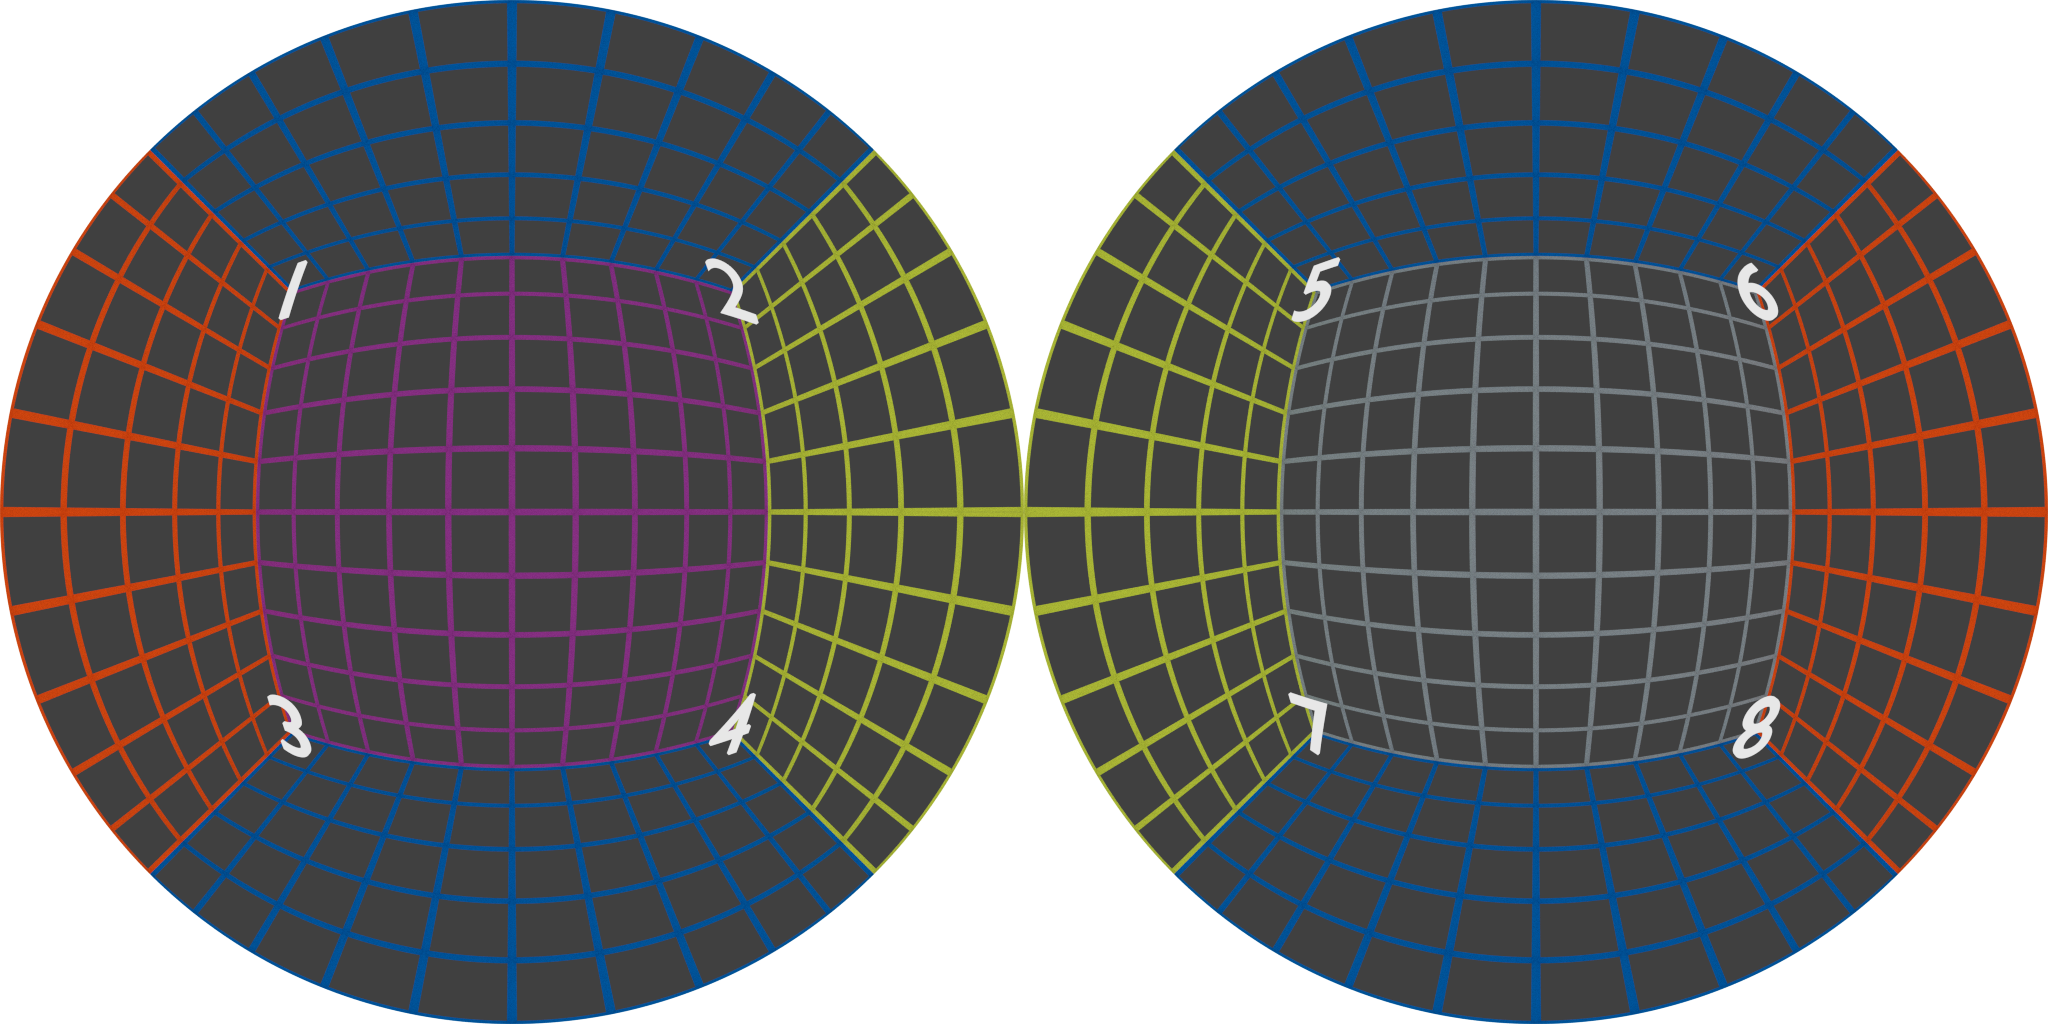
\includegraphics[width=1\textwidth]{figures/dfish.png}
				\caption{Vue sphérique \og dual fisheye \fg{}}
				\label{fig:dualfish}
			}
			\end{figure}
			\par
			On crée alors un rectangle où chaque pixel trouve un correspondant dans ces disques, et on obtient une projection equirectangulaire de l'espace sphérique d'origine. (\autoref{fig:equirect}).
			\begin{figure}[H]
			{
				\centering
				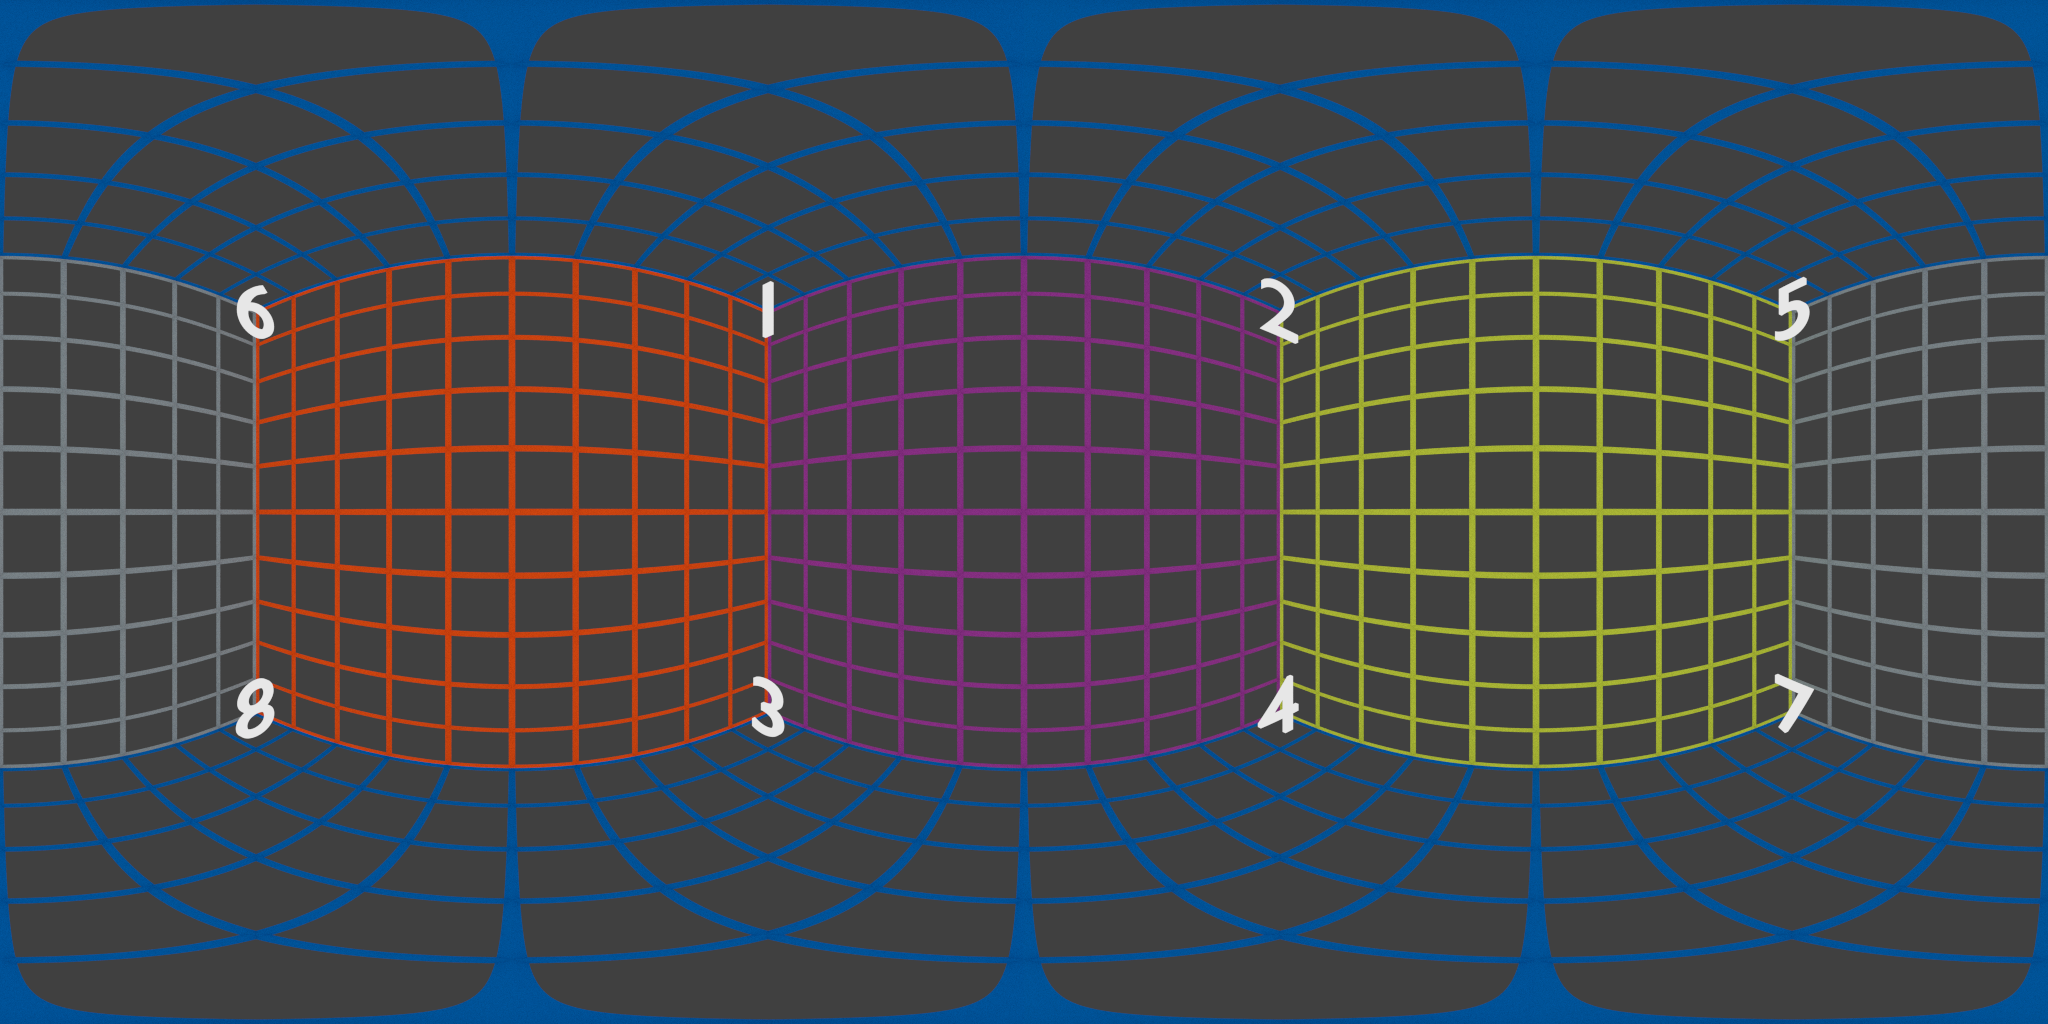
\includegraphics[width=1\textwidth]{figures/equirect.png}
				\caption{Projection equirectangulaire}
				\label{fig:equirect}
			}
			\end{figure}
			Bien qu'elles soient toujours déformées, les faces orange et verte deviennent assez linéaires pour présenter des caractéristiques spatiales détectables. On opère alors la détection sur cette image.
			\par
			L'opération mathématique correspondante revient à effectuer trois projections spatiales successives pour chaque pixel, ce qui justifie l'emploi du processeur graphique pour sa haute parallélisation des calculs.
			\par
			La première projection revient à retrouver les coordonnées sphériques réelles de l'objectif de la caméra à partir des coordonnées polaires des disques \emph{fisheye}. En effet, l'objectif est vu comme une hémisphère parfaite de rayon 1, afin de simplifier les calculs. Notons toutefois que l'objectif réel n'est pas une hémisphère parfaite, ce qui introduit l'utilisation de la distance focale dans les calculs afin de minimiser les déformations induites par cette approximation.
			\begin{figure}[htb]
				\centering
				\begin{minipage}{.5\textwidth}
					\centering
					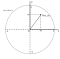
\includegraphics[width=0.95\linewidth]{figures/polar.pdf}
					\captionof{figure}{Coordonnées \newline cartésiennes sur image fisheye}
					\label{fig:pcart1}
				\end{minipage}%
				\begin{minipage}{.5\textwidth}
					\centering
					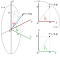
\includegraphics[width=0.95\linewidth]{figures/spherical.pdf}
					\captionof{figure}{Coordonnées sphériques (lentille de la caméra)}
					\label{fig:psph}
				\end{minipage}
			\end{figure}
			\par
			Le repère $(O,\vec{x},\vec{y})$ de la \autoref{fig:pcart1}, correspond à un disque de la photographie \emph{dual fisheye}, $O$ étant son centre.
			Le repère $(O,\vec{x},\vec{y},\vec{z})$ de la \autoref{fig:psph} correspond à l'espace réel de l'objectif de la caméra, avec $O'$ qui correspond au foyer focal du système optique.
			La correspondance entre ces repères est définie comme suit:
			\begin{center}
				$\forall P(x_{0},y_{0}) \in (O,\vec{x},\vec{y}), \exists P'(r,\theta,\phi) \in (O,\vec{x},\vec{y},\vec{z})$ avec $(x_{0},y_{0}) \in [-1;1]^2$ tel que: \newline
				$P'(x_{1},y_{1},z_{1}): \left\{
				\begin{array}{ll}
				\theta = \cos^{-1}{\left(\frac{x_{0}}{\sqrt{x_{0}^2+y_{0}^2}}\right)} \\
				\phi = \sin^{-1}{\left(\sqrt{x_{0}^2+y_{0}^2}\right)} \\
				r = 1
				\end{array}
				\right.\ $
			\end{center}
			L'étape suivante est d'utiliser les coordonnées cartésiennes de $P'$ afin d'obtenir la position (latitude, longitude) du point sur la sphère de l'espace de l'objectif de la caméra:
			\begin{center}
				$P'(x_{1},y_{1},z_{1}): \left\{
				\begin{array}{ll}
				x_{1} = r \sin \phi \cos \theta \\
				y_{1} = r \sin \phi \sin \theta \\
				z_{1} = r \cos \theta
				\end{array}
				\right.\ $ \newline \newline
				$ latitude = \tan^{-1}_{2}\left(y_{1}, x_{1}\right) $ \newline
				$ longitude = \tan^{-1}_{2}\left(z_{1}, \sqrt{x_{1}^2+y_{1}^2}\right) $ \newline
			\end{center}
			Finalement, on projette ces coordonnées depuis le plan sphérique sur un plan equirectangulaire:
			\begin{center}
				$P''(x_{2},y_{2}): \left\{
				\begin{array}{ll}
				x_{2} = \frac{longitude}{\pi} \\
				y_{2} = \frac{2 \times latitude}{\pi}
				\end{array}
				\right.\ $ \newline \newline
			\end{center}
		
			\begin{figure}[htb]
				\centering
				\begin{minipage}{.5\textwidth}
					\centering
					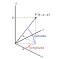
\includegraphics[width=0.95\linewidth]{figures/cartesian.pdf}
					\captionof{figure}{Latitude - longitude}
					\label{fig:platlong}
				\end{minipage}%
				\begin{minipage}{.5\textwidth}
					\centering
					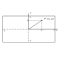
\includegraphics[width=0.95\linewidth]{figures/cart2.pdf}
					\captionof{figure}{Position equirectangulaire}
					\label{fig:pequirect}
				\end{minipage}
			\end{figure}
			\par
			
		\subsection{Détection et Classification}
		
			\content[inline]{A faire}
			
		\subsection{Présentation vidéo et incrustation}
		
		L'interface présentée en partie \ref{sub:ihm} s'occupe
		\begin{figure}[htb]
			\centering
			\begin{minipage}{.5\textwidth}
				\centering
				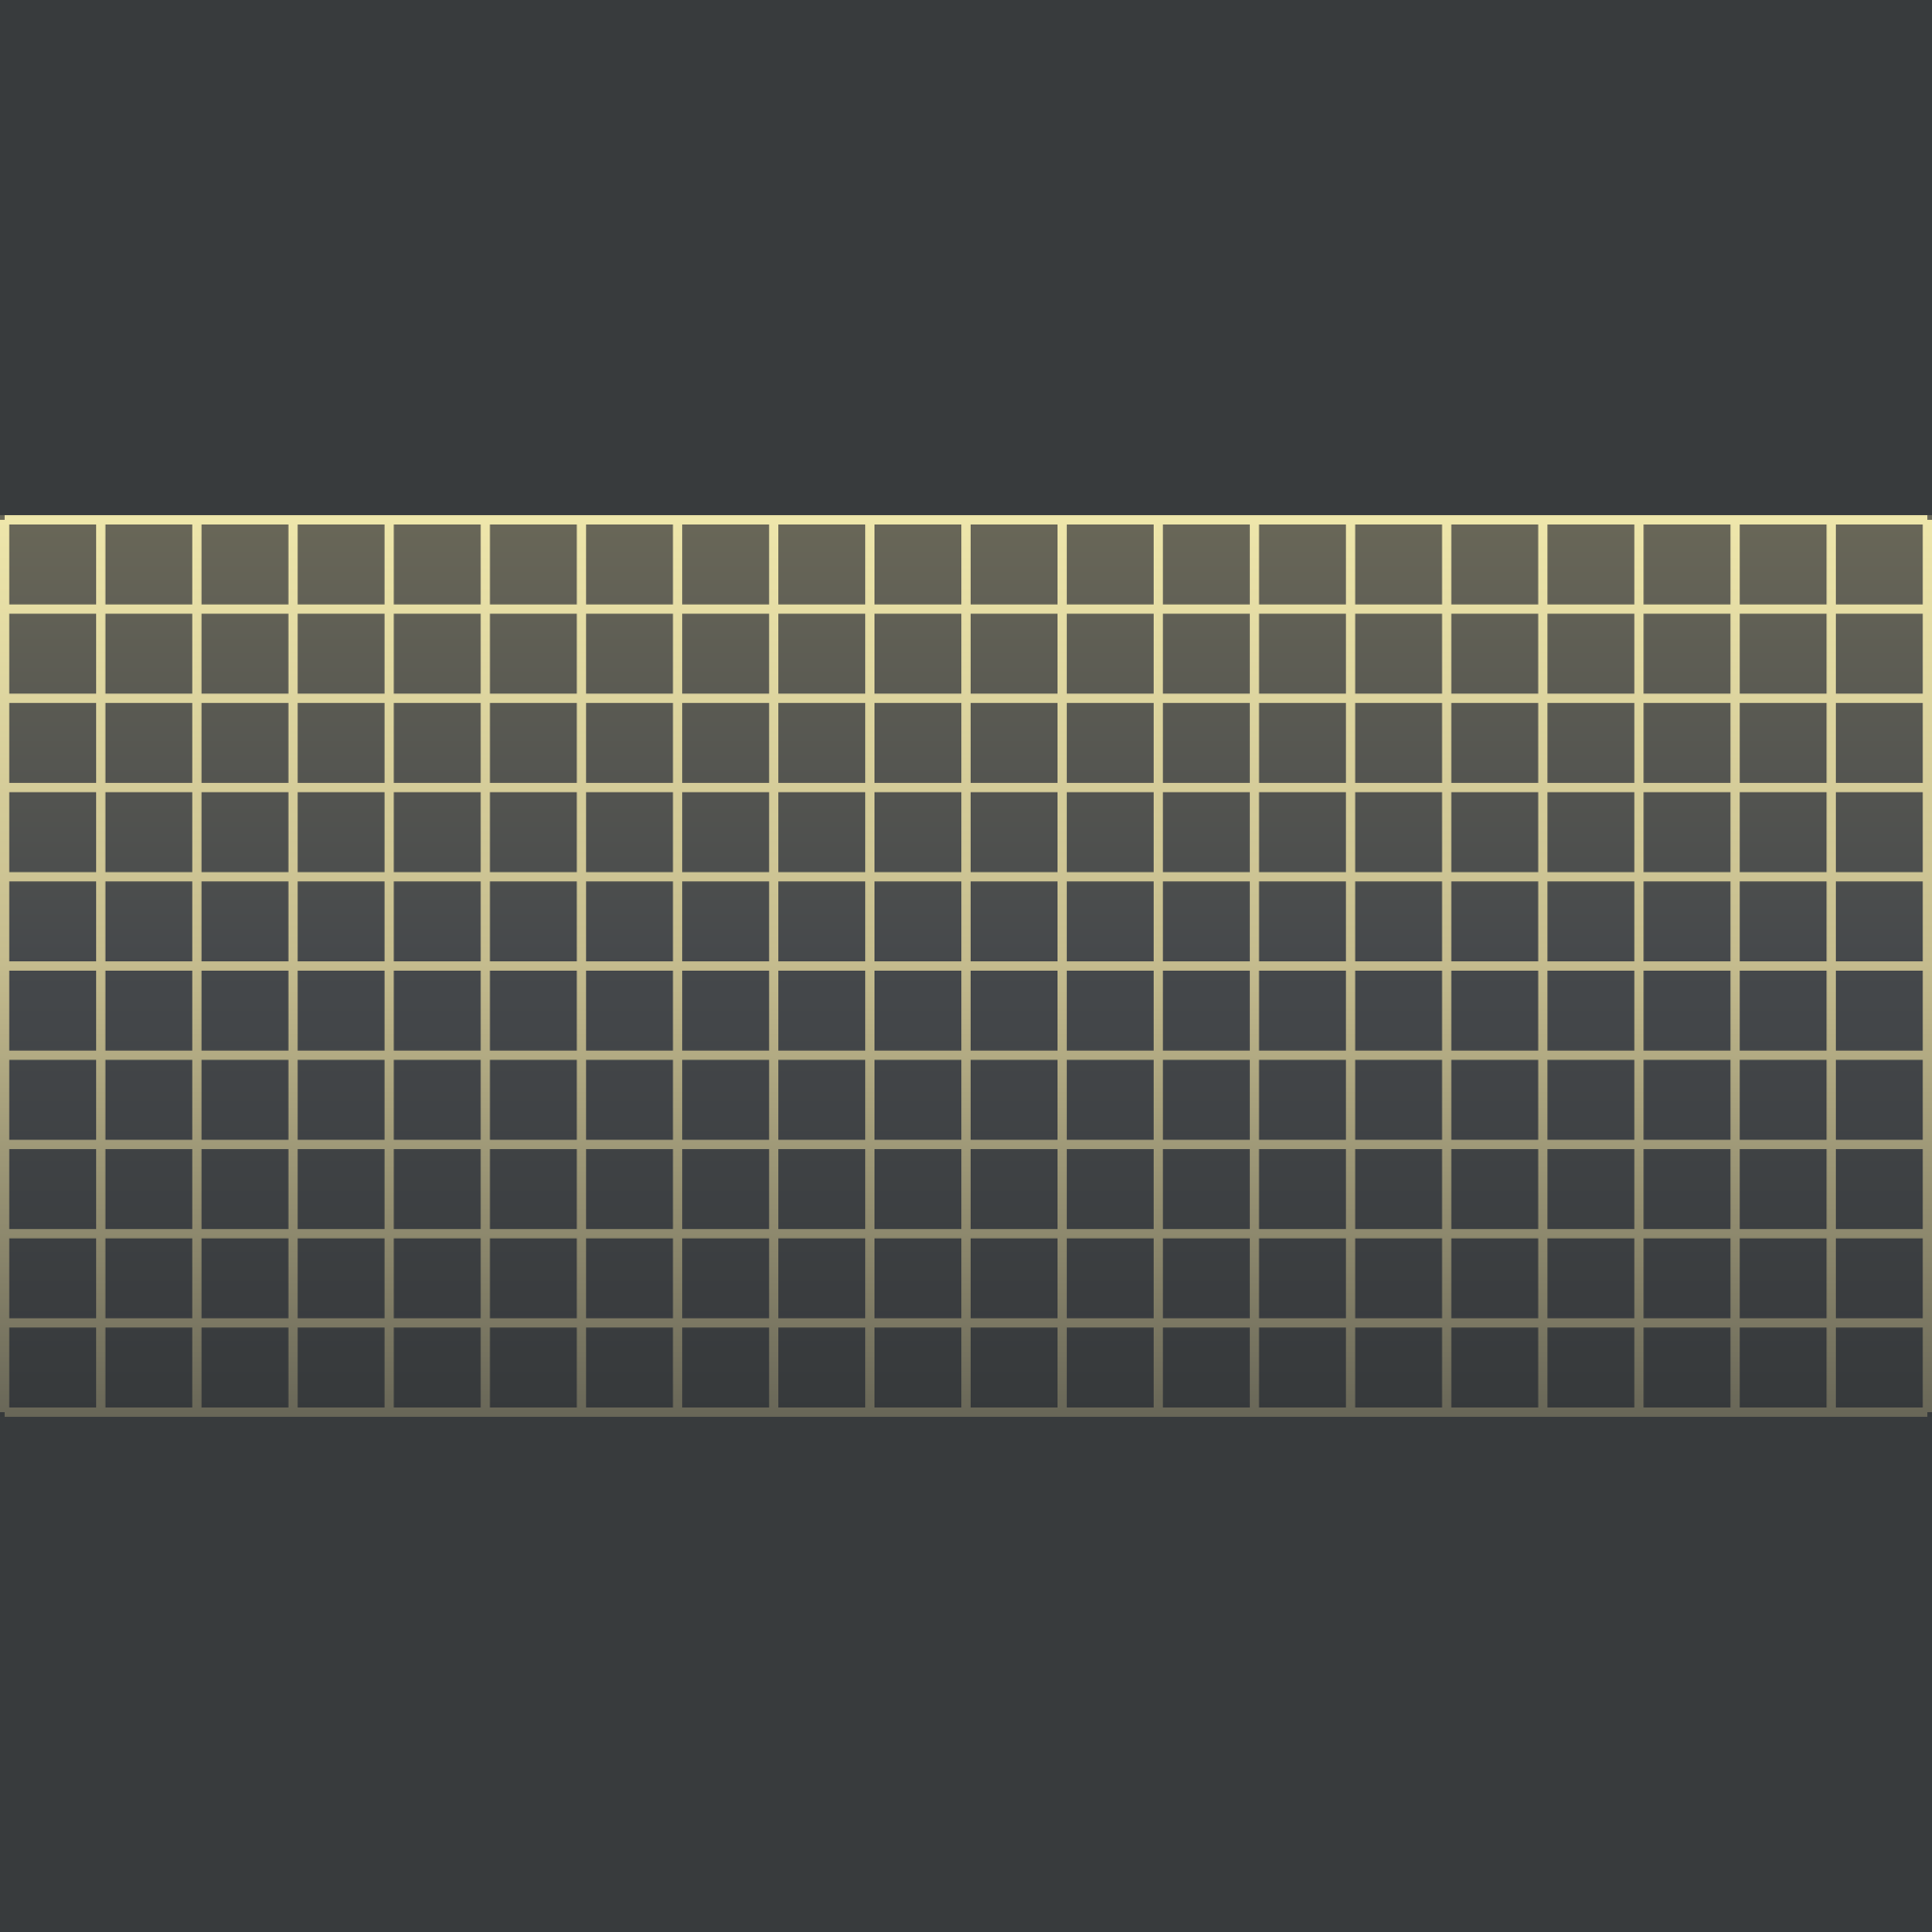
\includegraphics[width=0.95\linewidth]{figures/def0.png}
				\captionof{figure}{Image equirectangulaire}
				\label{fig:def0}
			\end{minipage}%
			\begin{minipage}{.5\textwidth}
				\centering
				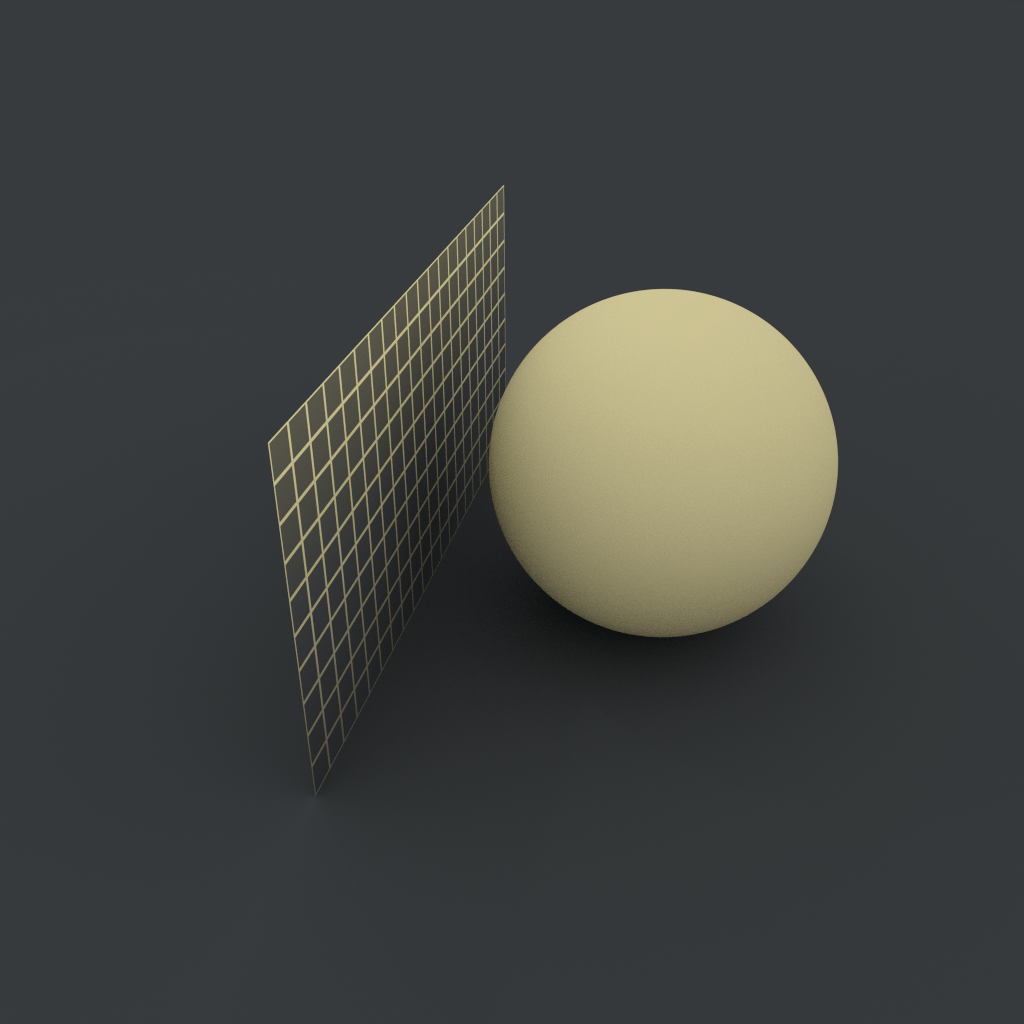
\includegraphics[width=0.95\linewidth]{figures/def1.png}
				\captionof{figure}{Texture mapping }
				\label{fig:def1}
			\end{minipage}
			
			\vspace{0.5cm}
			
			\begin{minipage}{.5\textwidth}
				\centering
				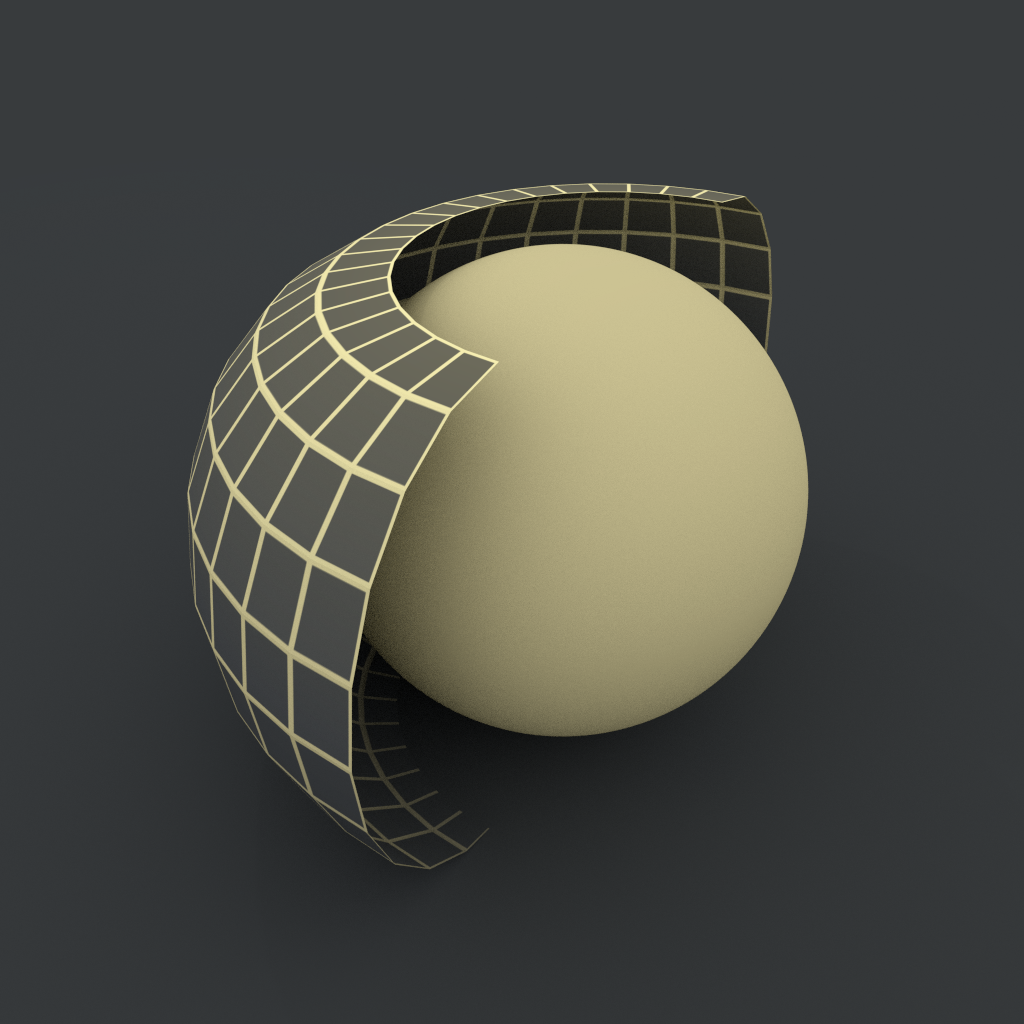
\includegraphics[width=0.95\linewidth]{figures/def2.png}
				\captionof{figure}{Déformation}
				\label{fig:def2}
			\end{minipage}%
			\begin{minipage}{.5\textwidth}
				\centering
				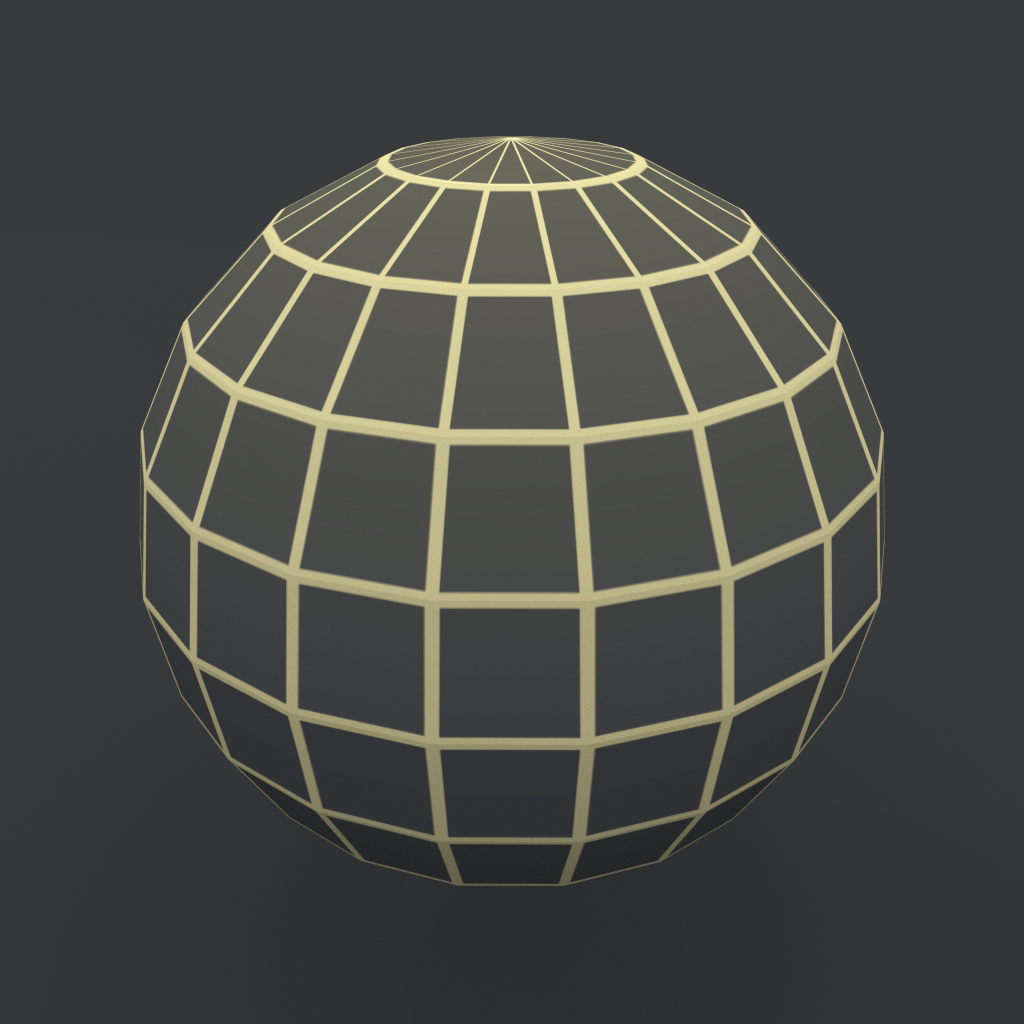
\includegraphics[width=0.95\linewidth]{figures/def3.png}
				\captionof{figure}{\emph{Sphere mapping}}
				\label{fig:def3}
			\end{minipage}
		\end{figure}
		\info[inline]{WIP}
			
		\subsection{Contrôle du robot}
		
			\content[inline]{A faire}
			
		\subsection{Modularité de l'IHM}
		
			\content[inline]{A faire}
			
	\section{Méthodes de travail}

		\subsection{Git-flow}
		
			\content[inline]{A faire}
			
		\subsection{Emprunts agiles}
		
			\content[inline]{A faire}
			

	\section{Pérennisation du projet}
	
		\subsection{Manuel utilisateur}
		
			Le projet est destiné à être poursuivi lors de stages ultérieurs, c'est pourquoi il a été décidé de rédiger un manuel d'utilisation, autant à l'intention des développeurs que pour un utilisateur \og opérateur \fg{}. Il regroupe un manuel d'installation, un guide de résolution des problèmes, un manuel d'utilisation de l'interface homme-machine et un guide de développement, qui explique le fonctionnement du logiciel et propose des améliorations possibles.
			\par
			Ce manuel a été rédigé en Markdown \cite{markdown}, un langage de balisage léger permettant une mise en forme rapide du texte et l'inclusion d'images. Il est compilé sous la forme d'un site html statique par MkDocs\cite{mkdocs}, ce qui permet une mise en forme agréable, ainsi qu'une navigation simple et plus intuitive qu'un document \og classique \fg{}. Il est donc prêt à être hébergé sur un serveur web.
			
		\subsection{Documentation}
		
			\content[inline]{A faire}
			
		\subsection{Installation automatique}
		
			\content[inline]{A faire}
				
		\subsection{Communication interne}
		
			\content[inline]{A faire}

	\chapter{Bilan et retour d'expérience}

	\section{Qualité des résultats}
	
		\content[inline]{A faire}

	\section{Perspectives d'évolution}
	
		\content[inline]{A faire}

	\section{Impact du projet}
		
		->nexter robotics
		\content[inline]{A faire}
	
	\section{Bilan personnel}
	
		\content[inline]{A faire}

	
	% Glossary
	\setglossarystyle{altlist}
	\printglossary[title={Glossaire}, toctitle={Glossaire}]
	\listoffigures
	
	% Bibliography
	\begin{thebibliography}{9}

	\bibitem{wikineuron}
		Wikipedia,
		\emph{Artificial neuron},
		\par
		\url{https://en.wikipedia.org/wiki/Artificial_neuron}.

	\bibitem{mscoco}
		Tsung-Yi Lin, Michael Maire, Serge Belongie, Lubomir Bourdev, Ross Girshick, James Hays, Pietro Perona, Deva Ramanan, C. Lawrence Zitnick, Piotr Dollár,
		\emph{Microsoft COCO: Common Objects in Context},
		21 fevrier 2015,
		\par
		\url{https://arxiv.org/abs/1405.0312}.

	\bibitem{ilsvrc}
		\emph{ILSVRC 2015: results},
		\par
		\url{http://image-net.org/challenges/LSVRC/2015/results}

\end{thebibliography}

	
	% Appendix
	\newpage
	\appendix
\chapter*{Annexes}
\newpage
\thispagestyle{empty}
\section*{Récapitulatif des caméras à images sphériques}

	\raisebox{-200mm}[0pt][0pt]
	{
		\hspace*{-1cm}
		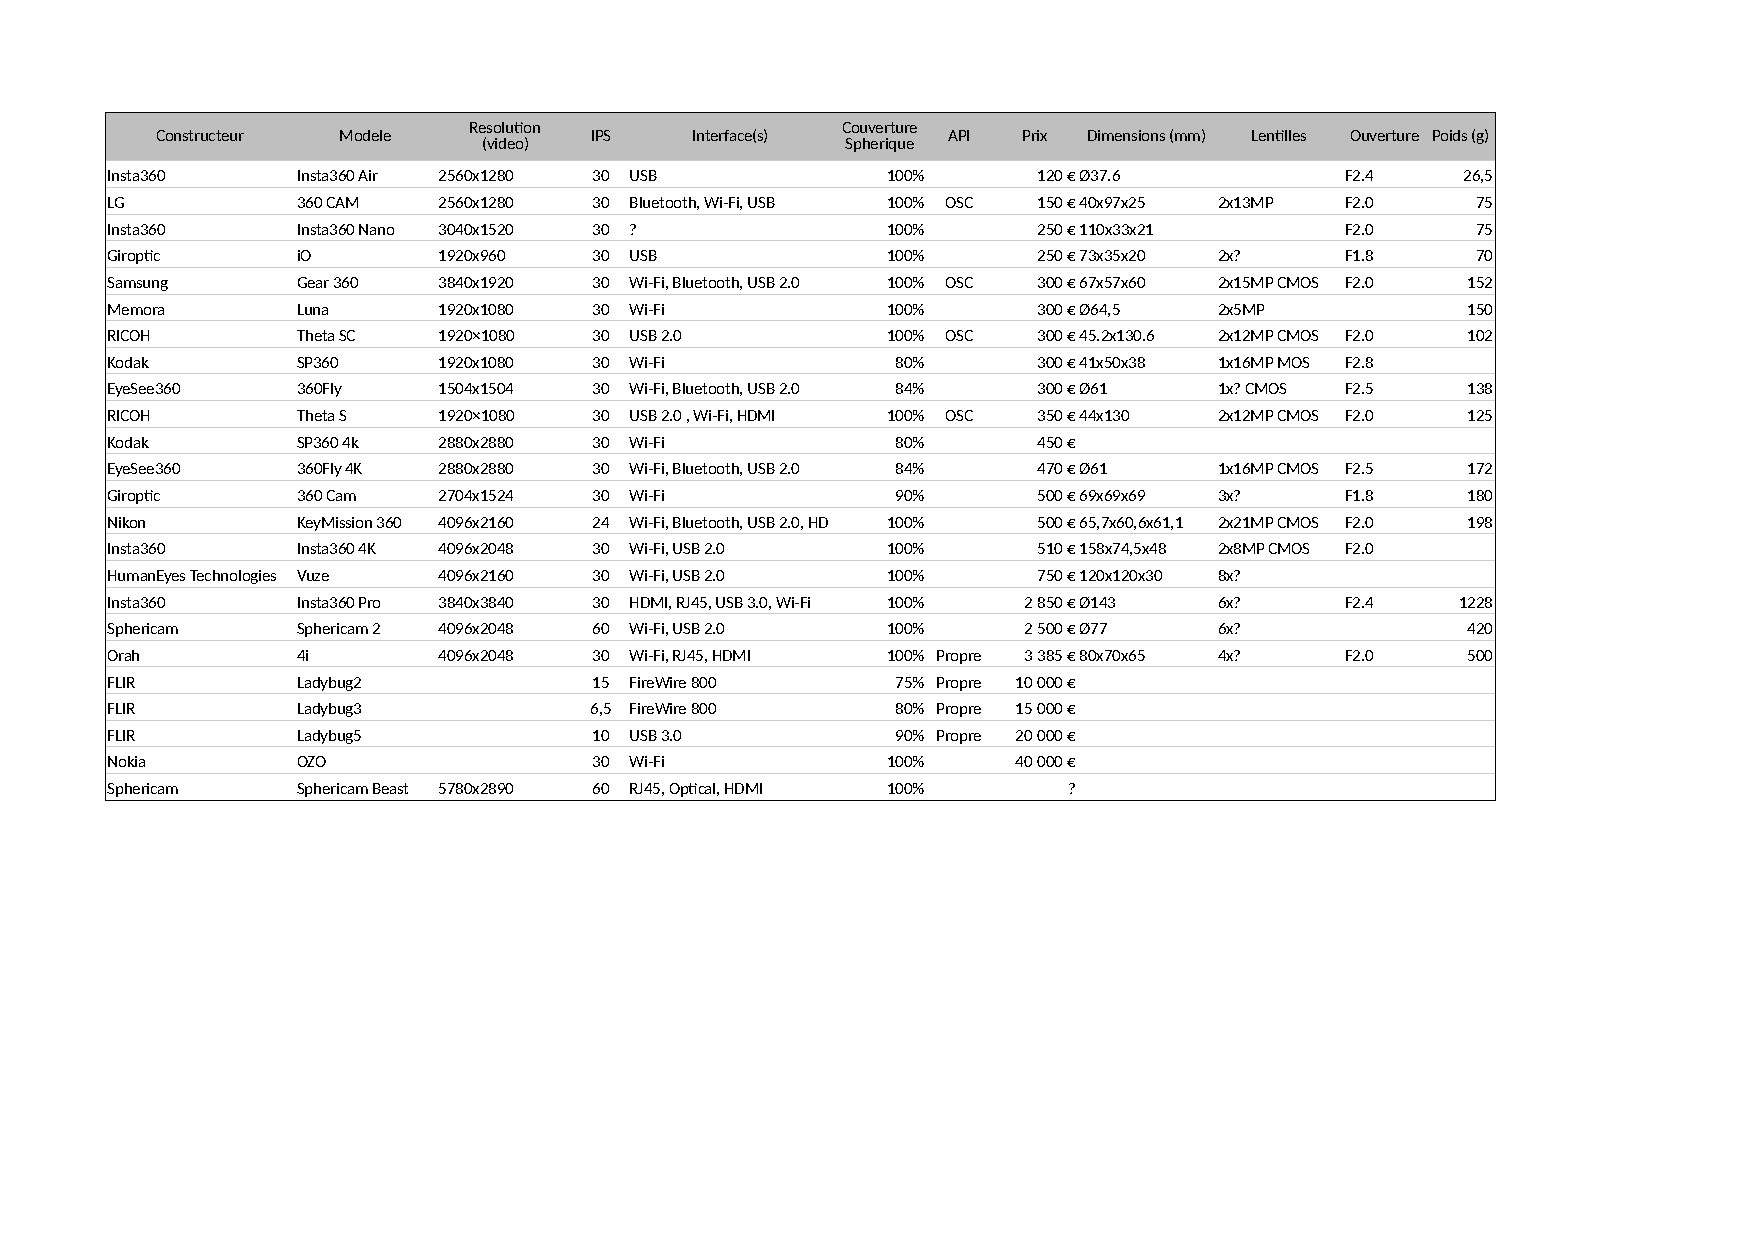
\includegraphics[angle=90,origin=c,scale=0.95]{premade/cameras_360.pdf}
	}

}
\end{document}
